\documentclass[12pt]{article}
\usepackage[margin=1in]{geometry}
\usepackage{graphicx}
\usepackage{amsmath}
\usepackage{tikz}
\usepackage{hyperref}
\usepackage{enumitem}

\newcommand{\fromlectures}{{\\ \color{blue} \hspace*{\fill}(from lecture slides)} \\}
\newcommand{\bydefn}{{\\ \color{blue} \hspace*{\fill}(by definition)} \\}
\newcommand{\given}{{\\ \color{blue} \hspace*{\fill}(given)} \\}
\newcommand{\rtp}{{\\ \color{blue} \hspace*{\fill}(required to prove)} \\}

\newcommand{\f}[1]{o_{#1}x_{#1}y_{#1}z_{#1}}
\newcommand{\rx}[1]{\begin{bmatrix} 1 & 0 & 0 & 0 \\ 0 & cos(#1) & -sin(#1) & 0 \\ 0 & sin(#1) & cos(#1) & 0 \\ 0 & 0 & 0 & 1 \end{bmatrix}}
\newcommand{\rz}[1]{\begin{bmatrix} cos(#1) & -sin(#1) & 0 & 0 \\ sin(#1) & cos(#1) & 0 & 0 \\ 0 & 0 & 1 & 0 \\ 0 & 0 & 0 & 1 \end{bmatrix}}
\newcommand{\iden}{\begin{bmatrix} 1 & 0 & 0 & 0 \\ 0 & 1 & 0 & 0 \\ 0 & 0 & 1 & 0 \\ 0 & 0 & 0 & 1 \end{bmatrix}}
\newcommand{\trans}[3]{\begin{bmatrix} 1 & 0 & 0 & #1 \\ 0 & 1 & 0 & #2 \\ 0 & 0 & 1 & #3 \\ 0 & 0 & 0 & 1 \end{bmatrix}}

\title{CSci 5551 - HW4}
\author{Yashasvi Sriram Patkuri\\patku001@umn.edu}

\begin{document}
\maketitle
\pagebreak

\section{}
A three link three joint planar robot with link lengths $l_1, l_2, l_3$ respectively is considered.
\given

\begin{figure}[h]
  \centering
  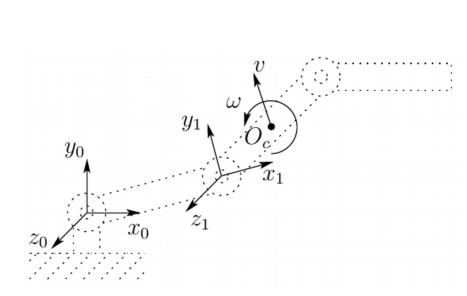
\includegraphics[width=0.6\textwidth]{q1.png}
  \caption{Three link three joint robot}
  \label{fig:q1.1}
\end{figure}
Assigning frames according to DH convention we have,
\fromlectures
\begin{figure}[h]
  \centering
  \begin{tikzpicture}[x=1cm, y=1cm, z=-0.6cm]
    % F0
    \draw [->]       (0, 0) -- (2, 0) node [right] {$x_0$};
    \draw            (0, 0) circle (0.15cm);
    \draw [fill]     (0, 0) circle (0.07cm) node [left] {$z_0$};
    % F1
    \draw [->]       (4, 2) -- (5.7888, 2.8944) node [right] {$x_1$};
    \draw            (4, 2) circle (0.15cm);
    \draw [fill]     (4, 2) circle (0.07cm) node [left] {$z_1$};
    % F2
    \draw [->]       (6, 5) -- (7.414, 6.414) node [right] {$x_2$};
    \draw            (6, 5) circle (0.15cm);
    \draw [fill]     (6, 5) circle (0.07cm) node [left] {$z_2$};
    % F3
    \draw [->]       (9, 5) -- (11, 5) node [right] {$x_3$};
    \draw            (9, 5) circle (0.15cm);
    \draw [fill]     (9, 5) circle (0.07cm) node [left] {$z_3$};
  \end{tikzpicture}
  \caption{DH frame assignment}
  \label{fig:q1.2}
\end{figure}

\begin{enumerate}[nolistsep]
  \item The z-axes are chosen along the axes of rotation and out of paper for the end-effector.
  \item The choice of $x_0$ is free so it is chosen to be parallel to ground for simplicity.
  \item There is a unique common normal b/w $z_0$ and $z_1$, along which $x_1$ is chosen.
  \item $x_2$ and $x_3$ are chosen in the same way.
\end{enumerate}

\subsubsection*{DH parameters}
The DH parameters for the frames shown in Figure \ref{fig:q1.2} are as follows
\begin{center}
\begin{tabular}{ c | c c c c }
 \hline
 $F_i \to F_j$ & $\theta$ & d & r & $\alpha$ \\
 \hline
 $0 \to 1$ & $\theta_1$ & 0 & $l_1$ & $0^{\circ}$ \\
 $1 \to 2$ & $\theta_2$ & 0 & $l_2$ & $0^{\circ}$ \\
 $2 \to 3$ & $\theta_3$ & 0 & $l_3$ & $0^{\circ}$ \\
 \hline
\end{tabular}
\end{center}

\subsubsection*{Finding transformation $T_{01}, T_{02}, T_{03}$}
Given frame i and frame j with DH parameters [ $\theta$, d, r, $\alpha$ ] the transformation matrix is
\[
  T_{i,j} \equiv Rot_{z,\theta} * Trans_{z, d} * Trans_{x, r} * Rot_{x, \alpha}
\]
\fromlectures
Consider $T_{01}$
\[
  T_{01} \equiv Rot_{z,\theta_1} * Trans_{z, 0} * Trans_{x, l_1} * Rot_{x, 0^{\circ}}
\]
\[
  T_{01} \equiv \rz{\theta_1} * \trans{0}{0}{0} * \trans{l_1}{0}{0} * \rx{0^{\circ}}
\]
\[
  T_{01} \equiv \rz{\theta_1} * \iden * \trans{l_1}{0}{0} * \iden
\]
\[
  T_{01} \equiv \rz{\theta_1} * \trans{l_1}{0}{0}
\]
\[
  T_{01} \equiv
  \begin{bmatrix} c_1 & -s_1 & 0 & l_1c_1 \\ s_1 & c_1 & 0 & l_1s_1 \\ 0 & 0 & 1 & 0 \\ 0 & 0 & 0 & 1 \end{bmatrix}
\]
Where $c_1 \equiv cos(\theta_1), s_1 \equiv sin(\theta_1)$.
$T_{12}, T_{23}$ have the same DH-parameter structure with changed variables, therefore we can use the final form of $T_{01}$ for them.
\[
  T_{12} \equiv
  \begin{bmatrix} c_2 & -s_2 & 0 & l_2c_2 \\ s_2 & c_2 & 0 & l_2s_2 \\ 0 & 0 & 1 & 0 \\ 0 & 0 & 0 & 1 \end{bmatrix}
\]
\[
  T_{23} \equiv
  \begin{bmatrix} c_3 & -s_3 & 0 & l_3c_3 \\ s_3 & c_3 & 0 & l_3s_3 \\ 0 & 0 & 1 & 0 \\ 0 & 0 & 0 & 1 \end{bmatrix}
\]
But
\[
  T_{ij} \equiv T_{ik} * T_{kj}
\]
\fromlectures
Therefore,
\[
  T_{02} \equiv T_{01} * T_{12}
\]
\[
  T_{02} \equiv
  \begin{bmatrix} c_1 & -s_1 & 0 & l_1c_1 \\ s_1 & c_1 & 0 & l_1s_1 \\ 0 & 0 & 1 & 0 \\ 0 & 0 & 0 & 1 \end{bmatrix}
  *
  \begin{bmatrix} c_2 & -s_2 & 0 & l_2c_2 \\ s_2 & c_2 & 0 & l_2s_2 \\ 0 & 0 & 1 & 0 \\ 0 & 0 & 0 & 1 \end{bmatrix}
\]
\[
  T_{02} \equiv
  \begin{bmatrix} c_1c_2 - s_1s_2 & -(s_1c_2 + c_1s_2) & 0 & l_1c_1 + l_2(c_1c_2 - s_1s_2) \\ s_1c_2 + c_1s_2 & c_1c_2 - s_1s_2 & 0 & l_1s_1 + l_2(s_1c_2 + c_1s_2) \\ 0 & 0 & 1 & 0 \\ 0 & 0 & 0 & 1 \end{bmatrix}
\]
\[
  T_{02} \equiv
  \begin{bmatrix} c_{12} & -s_{12} & 0 & l_1c_1 + l_2c_{12} \\ s_{12} & c_{12} & 0 & l_1s_1 + l_2s_{12} \\ 0 & 0 & 1 & 0 \\ 0 & 0 & 0 & 1 \end{bmatrix}
\]
Where $c_{12} \equiv cos(\theta_1 + \theta_2), s_{12} \equiv sin(\theta_1 + \theta_2)$.
Consider $T_{03}$,
\[
  T_{03} \equiv T_{02} * T_{23}
\]
\[
  T_{03} \equiv
  \begin{bmatrix} c_{12} & -s_{12} & 0 & l_1c_1 + l_2c_{12} \\ s_{12} & c_{12} & 0 & l_1s_1 + l_2s_{12} \\ 0 & 0 & 1 & 0 \\ 0 & 0 & 0 & 1 \end{bmatrix}
  *
  \begin{bmatrix} c_3 & -s_3 & 0 & l_3c_3 \\ s_3 & c_3 & 0 & l_3s_3 \\ 0 & 0 & 1 & 0 \\ 0 & 0 & 0 & 1 \end{bmatrix}
\]
\[
  T_{03} \equiv
  \begin{bmatrix}
    c_{12}c_{3} - s_{12}s_{3} & -(s_{12}c_{3} + c_{12}s_{3}) & 0 & l_1c_1 + l_2c_{12} + l_3(c_{12}c_{3} - s_{12}s_{3})\\
    s_{12}c_{3} + c_{12}s_{3} & c_{12}c_{3} - s_{12}s_{3}    & 0 & l_1s_1 + l_2s_{12} + l_3(s_{12}c_{3} + c_{12}s_{3})\\
    0 & 0 & 1 & 0 \\
    0 & 0 & 0 & 1
  \end{bmatrix}
\]
\[
  T_{03} \equiv
  \begin{bmatrix}
    c_{123} & -s_{123} & 0 & l_1c_1 + l_2c_{12} + l_3c_{123}\\
    s_{123} & c_{123}  & 0 & l_1s_1 + l_2s_{12} + l_3s_{123}\\
    0 & 0 & 1 & 0 \\
    0 & 0 & 0 & 1
  \end{bmatrix}
\]

\subsubsection*{Finding Jacobian}
For a 3R robot, the Jacobian of pose of end effector w.r.t frame 0 as a function of joint variables
\[
  J \equiv
  \begin{bmatrix} z_0^0 \times a_{03}^0 & z_1^0 \times a_{13}^0 & z_2^0 \times a_{23}^0 \\ z_0^0 & z_1^0 & z_2^0 \end{bmatrix}
\]
where
\[
  a_{i3}^{0} \equiv a_{3}^{0} - a_{i}^{0}
\]
where $a_3^0$ is the origin of frame 3 in frame 0 and $a_i^0$ is origin of frame i in frame 0.
$z_i^0$ can be obtained by the first three number of third column of $T_{0i}$.
\fromlectures
\[
  z_0^{0} \equiv z_1^{0} \equiv z_2^{0} \equiv z_3^{0} \equiv \begin{bmatrix} 0 \\ 0 \\ 1 \end{bmatrix}
\]
Consider $a_{3}^{0}$,
\[
  a_3^0 \equiv T_{03} * O_3
\]
\[
  a_3^0 \equiv
  \begin{bmatrix}
    c_{123} & -s_{123} & 0 & l_1c_1 + l_2c_{12} + l_3c_{123}\\
    s_{123} & c_{123}  & 0 & l_1s_1 + l_2s_{12} + l_3s_{123}\\
    0 & 0 & 1 & 0 \\
    0 & 0 & 0 & 1
  \end{bmatrix}
  *
  \begin{bmatrix} 0 \\ 0 \\ 0 \\ 1 \end{bmatrix}
\]
\[
  a_3^0 \equiv
  \begin{bmatrix}
    l_1c_1 + l_2c_{12} + l_3c_{123}\\
    l_1s_1 + l_2s_{12} + l_3s_{123}\\
    0 \\
    1
  \end{bmatrix}
\]
Consider $a_{2}^{0}$,
\[
  a_2^0 \equiv T_{02} * O_2
\]
\[
  a_2^0 \equiv
  \begin{bmatrix} c_{12} & -s_{12} & 0 & l_1c_1 + l_2c_{12} \\ s_{12} & c_{12} & 0 & l_1s_1 + l_2s_{12} \\ 0 & 0 & 1 & 0 \\ 0 & 0 & 0 & 1 \end{bmatrix}
  *
  \begin{bmatrix} 0 \\ 0 \\ 0 \\ 1 \end{bmatrix}
\]
\[
  a_2^0 \equiv
  \begin{bmatrix}
    l_1c_1 + l_2c_{12}\\
    l_1s_1 + l_2s_{12}\\
    0 \\
    1
  \end{bmatrix}
\]
Consider $a_{1}^{0}$,
\[
  a_1^0 \equiv T_{01} * O_1
\]
\[
  a_1^0 \equiv
  \begin{bmatrix} c_1 & -s_1 & 0 & l_1c_1 \\ s_1 & c_1 & 0 & l_1s_1 \\ 0 & 0 & 1 & 0 \\ 0 & 0 & 0 & 1 \end{bmatrix}
  *
  \begin{bmatrix} 0 \\ 0 \\ 0 \\ 1 \end{bmatrix}
\]
\[
  a_1^0 \equiv
  \begin{bmatrix}
    l_1c_1\\
    l_1s_1\\
    0 \\
    1
  \end{bmatrix}
\]
And,
\[
  a_0^0 \equiv \begin{bmatrix} 0 \\ 0 \\ 0 \\ 1 \end{bmatrix}
\]
Removing the homogeneous fourth coordinate we have,
\[
  a_0^0 \equiv
  \begin{bmatrix} 0 \\ 0 \\ 0  \end{bmatrix}
\]
\[
  a_1^0 \equiv
  \begin{bmatrix}
    l_1c_1\\
    l_1s_1\\
    0
  \end{bmatrix}
\]
\[
  a_2^0 \equiv
  \begin{bmatrix}
    l_1c_1 + l_2c_{12}\\
    l_1s_1 + l_2s_{12}\\
    0
  \end{bmatrix}
\]
\[
  a_3^0 \equiv
  \begin{bmatrix}
    l_1c_1 + l_2c_{12} + l_3c_{123}\\
    l_1s_1 + l_2s_{12} + l_3s_{123}\\
    0
  \end{bmatrix}
\]
Consider $a_{03}^0$,
\[
  a_{03}^0 \equiv a_3^0 - a_0^0
\]
\[
  a_{03}^0 \equiv
  \begin{bmatrix}
    l_1c_1 + l_2c_{12} + l_3c_{123}\\
    l_1s_1 + l_2s_{12} + l_3s_{123}\\
    0
  \end{bmatrix}
  -
  \begin{bmatrix} 0 \\ 0 \\ 0  \end{bmatrix}
\]
\[
  a_{03}^0 \equiv
  \begin{bmatrix}
    l_1c_1 + l_2c_{12} + l_3c_{123}\\
    l_1s_1 + l_2s_{12} + l_3s_{123}\\
    0
  \end{bmatrix}
\]
Consider $a_{13}^0$,
\[
  a_{13}^0 \equiv a_3^0 - a_1^0
\]
\[
  a_{13}^0 \equiv
  \begin{bmatrix}
    l_1c_1 + l_2c_{12} + l_3c_{123}\\
    l_1s_1 + l_2s_{12} + l_3s_{123}\\
    0
  \end{bmatrix}
  -
  \begin{bmatrix}
    l_1c_1\\
    l_1s_1\\
    0
  \end{bmatrix}
\]
\[
  a_{13}^0 \equiv
  \begin{bmatrix}
    l_2c_{12} + l_3c_{123}\\
    l_2s_{12} + l_3s_{123}\\
    0
  \end{bmatrix}
\]
Consider $a_{23}^0$,
\[
  a_{23}^0 \equiv a_3^0 - a_2^0
\]
\[
  a_{23}^0 \equiv
  \begin{bmatrix}
    l_1c_1 + l_2c_{12} + l_3c_{123}\\
    l_1s_1 + l_2s_{12} + l_3s_{123}\\
    0
  \end{bmatrix}
  -
  \begin{bmatrix}
    l_1c_1 + l_2c_{12}\\
    l_1s_1 + l_2s_{12}\\
    0
  \end{bmatrix}
\]
\[
  a_{23}^0 \equiv
  \begin{bmatrix}
    l_3c_{123}\\
    l_3s_{123}\\
    0
  \end{bmatrix}
\]
Consider the cross product of the form,
\[
  \begin{bmatrix} 0 \\ 0 \\ 1 \end{bmatrix} \times \begin{bmatrix} a \\ b \\ 0 \end{bmatrix}
  \equiv
  \begin{bmatrix} -b \\ a \\ 0 \end{bmatrix}
\]
Finally,
\[
  z_0^0 \times a_{03}^0 \equiv
  \begin{bmatrix} 0 \\ 0 \\ 1 \end{bmatrix} \times
  \begin{bmatrix}
    l_1c_1 + l_2c_{12} + l_3c_{123}\\
    l_1s_1 + l_2s_{12} + l_3s_{123}\\
    0
  \end{bmatrix}
  \equiv
  \begin{bmatrix}
    -(l_1s_1 + l_2s_{12} + l_3s_{123})\\
    l_1c_1 + l_2c_{12} + l_3c_{123}\\
    0
  \end{bmatrix}
\]
\[
  z_1^0 \times a_{13}^0 \equiv
  \begin{bmatrix} 0 \\ 0 \\ 1 \end{bmatrix} \times
  \begin{bmatrix}
    l_2c_{12} + l_3c_{123}\\
    l_2s_{12} + l_3s_{123}\\
    0
  \end{bmatrix}
  \equiv
  \begin{bmatrix}
    -(l_2s_{12} + l_3s_{123})\\
    l_2c_{12} + l_3c_{123}\\
    0
  \end{bmatrix}
\]
\[
  z_2^0 \times a_{23}^0 \equiv
  \begin{bmatrix} 0 \\ 0 \\ 1 \end{bmatrix} \times
  \begin{bmatrix}
    l_3c_{123}\\
    l_3s_{123}\\
    0
  \end{bmatrix}
  \equiv
  \begin{bmatrix}
    -(l_3s_{123})\\
    l_3c_{123}\\
    0
  \end{bmatrix}
\]
Using these to build the Jacobian,
\[
  J \equiv
  \begin{bmatrix}
    -(l_1s_1 + l_2s_{12} + l_3s_{123}) & -(l_2s_{12} + l_3s_{123}) & -(l_3s_{123})\\
    l_1c_1 + l_2c_{12} + l_3c_{123} & l_2c_{12} + l_3c_{123} & l_3c_{123}\\
    0 & 0 & 0 \\
    0 & 0 & 0 \\
    0 & 0 & 0 \\
    1 & 1 & 1 \\
  \end{bmatrix}
\]

\subsubsection*{Finding $v$ and $\omega$ of $O_c$}
The $v$ and $\omega$ of $O_c$ are not dependent on the last joint.
Consider a manipulator identical to the original one for the first one and half link.
The new manipulator will have its end-effector at $O_c$.
The required quantities can be found by repeating the same process of finding Jacobian as done for the original manipulator.

Assigning frames for the new manipulator according to DH convention we have,
\fromlectures
\begin{figure}[h]
  \centering
  \begin{tikzpicture}[x=1cm, y=1cm, z=-0.6cm]
    % F0
    \draw [->]       (0, 0) -- (2, 0) node [right] {$x_0$};
    \draw            (0, 0) circle (0.15cm);
    \draw [fill]     (0, 0) circle (0.07cm) node [left] {$z_0$};
    % F1
    \draw [->]       (4, 2) -- (5.7888, 2.8944) node [right] {$x_1$};
    \draw            (4, 2) circle (0.15cm);
    \draw [fill]     (4, 2) circle (0.07cm) node [left] {$z_1$};
    % F2
    \draw [->]       (5, 4) -- (6.414, 5.414) node [right] {$x_2$};
    \draw            (5, 4) circle (0.15cm);
    \draw [fill]     (5, 4) circle (0.07cm) node [left] {$z_2$};
  \end{tikzpicture}
  \caption{DH frame assignment}
  \label{fig:q1.3}
\end{figure}

\begin{enumerate}[nolistsep]
  \item The z-axes are chosen along the axes of rotation and out of paper for the end-effector.
  \item The choice of $x_0$ is free so it is chosen to be parallel to ground for simplicity.
  \item There is a unique common normal b/w $z_0$ and $z_1$, along which $x_1$ is chosen.
  \item $x_2$ is chosen in the same way.
\end{enumerate}

\subsubsection*{DH parameters}
The DH parameters for the frames shown in Figure \ref{fig:q1.3} are as follows
\begin{center}
\begin{tabular}{ c | c c c c }
 \hline
 $F_i \to F_j$ & $\theta$ & d & r & $\alpha$ \\
 \hline
 $0 \to 1$ & $\theta_1$ & 0 & $l_1$ & $0^{\circ}$ \\
 $1 \to 2$ & $\theta_2$ & 0 & $l_2 / 2$ & $0^{\circ}$ \\
 \hline
\end{tabular}
\end{center}

\subsubsection*{Finding transformation $T_{01}, T_{02}$}
Given frame i and frame j with DH parameters [ $\theta$, d, r, $\alpha$ ] the transformation matrix is
\[
  T_{i,j} \equiv Rot_{z,\theta} * Trans_{z, d} * Trans_{x, r} * Rot_{x, \alpha}
\]
\fromlectures
Consider $T_{01}$
\[
  T_{01} \equiv Rot_{z,\theta_1} * Trans_{z, 0} * Trans_{x, l_1} * Rot_{x, 0^{\circ}}
\]
\[
  T_{01} \equiv \rz{\theta_1} * \trans{0}{0}{0} * \trans{l_1}{0}{0} * \rx{0^{\circ}}
\]
\[
  T_{01} \equiv \rz{\theta_1} * \iden * \trans{l_1}{0}{0} * \iden
\]
\[
  T_{01} \equiv \rz{\theta_1} * \trans{l_1}{0}{0}
\]
\[
  T_{01} \equiv
  \begin{bmatrix} c_1 & -s_1 & 0 & l_1c_1 \\ s_1 & c_1 & 0 & l_1s_1 \\ 0 & 0 & 1 & 0 \\ 0 & 0 & 0 & 1 \end{bmatrix}
\]
Where $c_1 \equiv cos(\theta_1), s_1 \equiv sin(\theta_1)$.
$T_{12}$ has the same DH-parameter structure with changed variables, therefore we can use the final form of $T_{01}$ for it.
\[
  T_{12} \equiv
  \begin{bmatrix} c_2 & -s_2 & 0 & \frac{l_2}{2}c_2 \\ s_2 & c_2 & 0 & \frac{l_2}{2}s_2 \\ 0 & 0 & 1 & 0 \\ 0 & 0 & 0 & 1 \end{bmatrix}
\]
But
\[
  T_{ij} \equiv T_{ik} * T_{kj}
\]
\fromlectures
Therefore,
\[
  T_{02} \equiv T_{01} * T_{12}
\]
\[
  T_{02} \equiv
  \begin{bmatrix} c_1 & -s_1 & 0 & l_1c_1 \\ s_1 & c_1 & 0 & l_1s_1 \\ 0 & 0 & 1 & 0 \\ 0 & 0 & 0 & 1 \end{bmatrix}
  *
  \begin{bmatrix} c_2 & -s_2 & 0 & \frac{l_2}{2}c_2 \\ s_2 & c_2 & 0 & \frac{l_2}{2}s_2 \\ 0 & 0 & 1 & 0 \\ 0 & 0 & 0 & 1 \end{bmatrix}
\]
\[
  T_{02} \equiv
  \begin{bmatrix} c_1c_2 - s_1s_2 & -(s_1c_2 + c_1s_2) & 0 & l_1c_1 + \frac{l_2}{2}(c_1c_2 - s_1s_2) \\ s_1c_2 + c_1s_2 & c_1c_2 - s_1s_2 & 0 & l_1s_1 + \frac{l_2}{2}(s_1c_2 + c_1s_2) \\ 0 & 0 & 1 & 0 \\ 0 & 0 & 0 & 1 \end{bmatrix}
\]
\[
  T_{02} \equiv
  \begin{bmatrix} c_{12} & -s_{12} & 0 & l_1c_1 + \frac{l_2}{2}c_{12} \\ s_{12} & c_{12} & 0 & l_1s_1 + \frac{l_2}{2}s_{12} \\ 0 & 0 & 1 & 0 \\ 0 & 0 & 0 & 1 \end{bmatrix}
\]
Where $c_{12} \equiv cos(\theta_1 + \theta_2), s_{12} \equiv sin(\theta_1 + \theta_2)$.

\subsubsection*{Finding Jacobian}
For a 2R robot, the Jacobian of pose of end effector w.r.t frame 0 as a function of joint variables
\[
  J \equiv
  \begin{bmatrix} z_0^0 \times a_{02}^0 & z_1^0 \times a_{12}^0\\ z_0^0 & z_1^0 \end{bmatrix}
\]
where
\[
  a_{i2}^{0} \equiv a_{2}^{0} - a_{i}^{0}
\]
where $a_2^0$ is the origin of frame 2 in frame 0 and $a_i^0$ is origin of frame i in frame 0.
$z_i^0$ can be obtained by the first three number of third column of $T_{0i}$.
\fromlectures
\[
  z_0^{0} \equiv z_1^{0} \equiv z_2^{0} \equiv \begin{bmatrix} 0 \\ 0 \\ 1 \end{bmatrix}
\]
Consider $a_{2}^{0}$,
\[
  a_2^0 \equiv T_{02} * O_2
\]
\[
  a_2^0 \equiv
  \begin{bmatrix}
    c_{12} & -s_{12} & 0 & l_1c_1 + \frac{l_2}{2}c_{12}\\
    s_{12} & c_{12} & 0 & l_1s_1 + \frac{l_2}{2}s_{12} \\
    0 & 0 & 1 & 0 \\
    0 & 0 & 0 & 1
  \end{bmatrix}
  *
  \begin{bmatrix} 0 \\ 0 \\ 0 \\ 1 \end{bmatrix}
\]
\[
  a_2^0 \equiv
  \begin{bmatrix}
    l_1c_1 + \frac{l_2}{2}c_{12}\\
    l_1s_1 + \frac{l_2}{2}s_{12} \\
    0 \\
    1
  \end{bmatrix}
\]
Consider $a_{1}^{0}$,
\[
  a_1^0 \equiv T_{01} * O_1
\]
\[
  a_1^0 \equiv
  \begin{bmatrix} c_1 & -s_1 & 0 & l_1c_1 \\ s_1 & c_1 & 0 & l_1s_1 \\ 0 & 0 & 1 & 0 \\ 0 & 0 & 0 & 1 \end{bmatrix}
  *
  \begin{bmatrix} 0 \\ 0 \\ 0 \\ 1 \end{bmatrix}
\]
\[
  a_1^0 \equiv
  \begin{bmatrix}
    l_1c_1\\
    l_1s_1\\
    0 \\
    1
  \end{bmatrix}
\]
And,
\[
  a_0^0 \equiv \begin{bmatrix} 0 \\ 0 \\ 0 \\ 1 \end{bmatrix}
\]
Removing the homogeneous fourth coordinate we have,
\[
  a_0^0 \equiv
  \begin{bmatrix} 0 \\ 0 \\ 0  \end{bmatrix}
\]
\[
  a_1^0 \equiv
  \begin{bmatrix}
    l_1c_1\\
    l_1s_1\\
    0
  \end{bmatrix}
\]
\[
  a_2^0 \equiv
  \begin{bmatrix}
    l_1c_1 + \frac{l_2}{2}c_{12}\\
    l_1s_1 + \frac{l_2}{2}s_{12}\\
    0
  \end{bmatrix}
\]
Consider $a_{02}^0$,
\[
  a_{02}^0 \equiv a_2^0 - a_0^0
\]
\[
  a_{02}^0 \equiv
  \begin{bmatrix}
    l_1c_1 + \frac{l_2}{2}c_{12}\\
    l_1s_1 + \frac{l_2}{2}s_{12}\\
    0
  \end{bmatrix}
  -
  \begin{bmatrix} 0 \\ 0 \\ 0  \end{bmatrix}
\]
\[
  a_{02}^0 \equiv
  \begin{bmatrix}
    l_1c_1 + \frac{l_2}{2}c_{12}\\
    l_1s_1 + \frac{l_2}{2}s_{12}\\
    0
  \end{bmatrix}
\]
Consider $a_{12}^0$,
\[
  a_{12}^0 \equiv a_2^0 - a_1^0
\]
\[
  a_{12}^0 \equiv
  \begin{bmatrix}
    l_1c_1 + \frac{l_2}{2}c_{12}\\
    l_1s_1 + \frac{l_2}{2}s_{12}\\
    0
  \end{bmatrix}
  -
  \begin{bmatrix}
    l_1c_1\\
    l_1s_1\\
    0
  \end{bmatrix}
\]
\[
  a_{12}^0 \equiv
  \begin{bmatrix}
    \frac{l_2}{2}c_{12}\\
    \frac{l_2}{2}s_{12}\\
    0
  \end{bmatrix}
\]
Consider the cross product of the form,
\[
  \begin{bmatrix} 0 \\ 0 \\ 1 \end{bmatrix} \times \begin{bmatrix} a \\ b \\ 0 \end{bmatrix}
  \equiv
  \begin{bmatrix} -b \\ a \\ 0 \end{bmatrix}
\]
Finally,
\[
  z_0^0 \times a_{02}^0 \equiv
  \begin{bmatrix} 0 \\ 0 \\ 1 \end{bmatrix} \times
  \begin{bmatrix}
    l_1c_1 + \frac{l_2}{2}c_{12}\\
    l_1s_1 + \frac{l_2}{2}s_{12}\\
    0
  \end{bmatrix}
  \equiv
  \begin{bmatrix}
    -(l_1s_1 + \frac{l_2}{2}s_{12})\\
    l_1c_1 + \frac{l_2}{2}c_{12}\\
    0
  \end{bmatrix}
\]
\[
  z_1^0 \times a_{12}^0 \equiv
  \begin{bmatrix} 0 \\ 0 \\ 1 \end{bmatrix} \times
  \begin{bmatrix}
    \frac{l_2}{2}c_{12}\\
    \frac{l_2}{2}s_{12}\\
    0
  \end{bmatrix}
  \equiv
  \begin{bmatrix}
    -(\frac{l_2}{2}s_{12})\\
    \frac{l_2}{2}c_{12}\\
    0
  \end{bmatrix}
\]
Using these to build the Jacobian,
\[
  J \equiv
  \begin{bmatrix}
    -(l_1s_1 + \frac{l_2}{2}s_{12}) & -(\frac{l_2}{2}s_{12})\\
    l_1c_1 + \frac{l_2}{2}c_{12} & \frac{l_2}{2}c_{12}\\
    0 & 0 \\
    0 & 0 \\
    0 & 0 \\
    1 & 1 \\
  \end{bmatrix}
\]
Finally,
\[
  \begin{bmatrix} v \\ \omega \end{bmatrix}
  \equiv
  J *
  \begin{bmatrix} \frac{d\theta_1}{dt} \\ \frac{d\theta_2}{dt} \end{bmatrix}
\]
\[
  \begin{bmatrix} v \\ \omega \end{bmatrix}
  \equiv
  \begin{bmatrix}
    -(l_1s_1 + \frac{l_2}{2}s_{12}) & -(\frac{l_2}{2}s_{12})\\
    l_1c_1 + \frac{l_2}{2}c_{12} & \frac{l_2}{2}c_{12}\\
    0 & 0 \\
    0 & 0 \\
    0 & 0 \\
    1 & 1 \\
  \end{bmatrix}
  *
  \begin{bmatrix} \frac{d\theta_1}{dt} \\ \frac{d\theta_2}{dt} \end{bmatrix}
\]
\[
  \begin{bmatrix} v \\ \omega \end{bmatrix}
  \equiv
  \begin{bmatrix}
    -(l_1s_1 + \frac{l_2}{2}s_{12}) * \frac{d\theta_1}{dt} - (\frac{l_2}{2}s_{12}) * \frac{d\theta_2}{dt} \\
    l_1c_1 + \frac{l_2}{2}c_{12} * \frac{d\theta_1}{dt} + \frac{l_2}{2}c_{12} * \frac{d\theta_2}{dt}\\
    0 \\
    0 \\
    0 \\
    \frac{d\theta_1}{dt} + \frac{d\theta_2}{dt}\\
  \end{bmatrix}
\]
Therefore,
\[
  v
  \equiv
  \begin{bmatrix}
    -(l_1s_1 + \frac{l_2}{2}s_{12}) * \frac{d\theta_1}{dt} - \frac{l_2}{2}s_{12} * \frac{d\theta_2}{dt} \\
    (l_1c_1 + \frac{l_2}{2}c_{12}) * \frac{d\theta_1}{dt} + \frac{l_2}{2}c_{12} * \frac{d\theta_2}{dt}\\
    0 \\
  \end{bmatrix},
  \omega
  \equiv
  \begin{bmatrix}
    0 \\
    0 \\
    \frac{d\theta_1}{dt} + \frac{d\theta_2}{dt}\\
  \end{bmatrix}
\]

\pagebreak

\section{}
A three link three joint robot with link lengths $l_1, l_2, l_3$ respectively is considered.
\given
\begin{figure}[h]
  \centering
  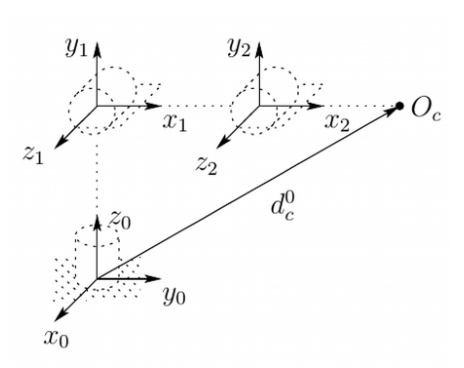
\includegraphics[width=0.6\textwidth]{q2.png}
  \caption{Three link three joint robot}
  \label{fig:q2.1}
\end{figure}
\begin{figure}[h]
  \centering
  \begin{tikzpicture}[x=1cm, y=1cm, z=-0.6cm]
    \draw [dashed, red]       (-3, 0) -- (-3, 3) node [right] {$l_1$};
    \draw [dashed, red]       (0, 5) -- (3, 5) node [right] {$l_2$};
    \draw [dashed, red]       (3, 4) -- (6, 4) node [right] {$l_3$};
    % F0
    \draw [->]       (0, 0) -- (0, 1) node [right] {$z_0$};
    \draw            (0, 0) circle (0.15cm);
    \draw [fill]     (0, 0) circle (0.07cm) node [left] {$x_0$};
    % F1
    \draw [->]       (0, 3) -- (1, 3) node [right] {$x_1$};
    \draw            (0, 3) circle (0.15cm);
    \draw [fill]     (0, 3) circle (0.07cm) node [left] {$z_1$};
    % F2
    \draw [->]       (3, 3) -- (4, 3) node [right] {$x_2$};
    \draw            (3, 3) circle (0.15cm);
    \draw [fill]     (3, 3) circle (0.07cm) node [left] {$z_2$};
    % F3
    \draw [->]       (6, 3) -- (7, 3) node [right] {$x_3$};
    \draw            (6, 3) circle (0.15cm);
    \draw [fill]     (6, 3) circle (0.07cm) node [left] {$z_3$};
  \end{tikzpicture}
  \caption{DH frame assignment}
  \label{fig:q2.2}
\end{figure}
\pagebreak

\subsubsection*{DH parameters}
The DH parameters for the frames shown in Figure \ref{fig:q2.2} are as follows
\begin{center}
\begin{tabular}{ c | c c c c }
 \hline
 $F_i \to F_j$ & $\theta$ & d & r & $\alpha$ \\
 \hline
 $0 \to 1$ & $\theta_1$ & $l_1$ & $ 0 $ & $90^{\circ}$ \\
 $1 \to 2$ & $\theta_2$ & 0     & $l_2$ & $0^{\circ}$ \\
 $2 \to 3$ & $\theta_3$ & 0     & $l_3$ & $0^{\circ}$ \\
 \hline
\end{tabular}
\end{center}

\subsubsection*{Finding transformation $T_{01}, T_{02}, T_{03}$}
Given frame i and frame j with DH parameters [ $\theta$, d, r, $\alpha$ ] the transformation matrix is
\[
  T_{i,j} \equiv Rot_{z,\theta} * Trans_{z, d} * Trans_{x, r} * Rot_{x, \alpha}
\]
\fromlectures
Consider $T_{01}$
\[
  T_{01} \equiv Rot_{z,\theta_1} * Trans_{z, l_1} * Trans_{x, 0} * Rot_{x, 90^{\circ}}
\]
\[
  T_{01} \equiv Rot_{z,\theta_1} * Trans_{z, l_1} * \iden * Rot_{x, 90^{\circ}}
\]
\[
  T_{01} \equiv Rot_{z,\theta_1} * Trans_{z, l_1} * Rot_{x, 90^{\circ}}
\]
\[
  T_{01} \equiv \rz{\theta_1} * \trans{0}{0}{l_1} * \rx{90^{\circ}}
\]
\[
  T_{01} \equiv
  \begin{bmatrix}
    c_1 & -s_1 & 0 & 0 \\
    s_1 & c_1 & 0 & 0 \\
    0 & 0 & 1 & l_1 \\
    0 & 0 & 0 & 1
  \end{bmatrix} * \rx{90^{\circ}}
\]
where $c_i \equiv cos(\theta_i), s_i \equiv sin(\theta_i)$.
\[
  T_{01} \equiv
  \begin{bmatrix}
    c_1 & 0 & s_1 & 0 \\
    s_1 & 0 & -c_1 & 0 \\
    0 & 1 & 0 & l_1 \\
    0 & 0 & 0 & 1
  \end{bmatrix}
\]
Consider $T_{12}$
\[
  T_{12} \equiv Rot_{z,\theta_2} * Trans_{z, 0} * Trans_{x, l_2} * Rot_{x, 0^{\circ}}
\]
\[
  T_{12} \equiv \rz{\theta_2} * \iden * \trans{l_2}{0}{0} * \rx{0^{\circ}}
\]
\[
  T_{12} \equiv \rz{\theta_2} * \iden * \trans{l_2}{0}{0} * \iden
\]
\[
  T_{12} \equiv \rz{\theta_2} * \trans{l_2}{0}{0}
\]
\[
  T_{12} \equiv
  \begin{bmatrix}
    c_2 & -s_2 & 0 & l_2c_2 \\
    s_2 & c_2 & 0 & l_2s_2 \\
    0 & 0 & 1 & 0 \\
    0 & 0 & 0 & 1
  \end{bmatrix}
\]
$T_{23}$ has same DH structure as $T_{12}$, therefore we can use the final form of the latter. Therefore,
\[
  T_{23} \equiv
  \begin{bmatrix}
    c_3 & -s_3 & 0 & l_3c_3 \\
    s_3 & c_3 & 0 & l_3s_3 \\
    0 & 0 & 1 & 0 \\
    0 & 0 & 0 & 1
  \end{bmatrix}
\]
But
\[
  T_{ij} \equiv T_{ik} * T_{kj}
\]
\fromlectures
Therefore,
\[
  T_{02} \equiv T_{01} * T_{12}
\]
\[
  T_{02} \equiv
  \begin{bmatrix}
    c_1 & 0 & s_1 & 0 \\
    s_1 & 0 & -c_1 & 0 \\
    0 & 1 & 0 & l_1 \\
    0 & 0 & 0 & 1
  \end{bmatrix}
  *
  \begin{bmatrix}
    c_2 & -s_2 & 0 & l_2c_2 \\
    s_2 & c_2 & 0 & l_2s_2 \\
    0 & 0 & 1 & 0 \\
    0 & 0 & 0 & 1
  \end{bmatrix}
\]
\[
  T_{02} \equiv
  \begin{bmatrix}
    c_1c_2 & -c_1s_2 & s_1 & l_2c_1c_2 \\
    s_1c_2 & -s_1s_2 & -c_1 & l_2s_1c_2 \\
    s_2 & c_2 & 0 & l_2s_2 + l_1 \\
    0 & 0 & 0 & 1
  \end{bmatrix}
\]
\[
  T_{03} \equiv T_{02} * T_{23}
\]
\[
  T_{03} \equiv
  \begin{bmatrix}
    c_1c_2 & -c_1s_2 & s_1 & l_2c_1c_2 \\
    s_1c_2 & -s_1s_2 & -c_1 & l_2s_1c_2 \\
    s_2 & c_2 & 0 & l_2s_2 + l_1 \\
    0 & 0 & 0 & 1
  \end{bmatrix}
  *
  \begin{bmatrix}
    c_3 & -s_3 & 0 & l_3c_3 \\
    s_3 & c_3 & 0 & l_3s_3 \\
    0 & 0 & 1 & 0 \\
    0 & 0 & 0 & 1
  \end{bmatrix}
\]
\[
  T_{03} \equiv
  \begin{bmatrix}
    c_1(c_2c_3 - s_2s_3) & -c_1(s_2c_3 + c_2s_3) & s_1  & c_1l_2c_2 + c_1l_3(c_2c_3 - s_2s_3) \\
    s_2(c_2c_3 - s_2s_3) & -s_1(s_2c_3 + c_2s_3) & -c_1 & s_1l_2c_2 + s_1l_3(c_2c_3 - s_2s_3) \\
    s_2c_3 + c_2s_3      & c_2c_3 - s_2s_3       & 0    & l_2s_2 + l_3(s_2c_3 + c_2s_3) + l_1 \\
    0 & 0 & 0 & 1
  \end{bmatrix}
\]
\[
  T_{03} \equiv
  \begin{bmatrix}
    c_1c_{23} & -c_1s_{23} & s_1  & l_2c_1c_2 + l_3c_1c_{23} \\
    s_1c_{23} & -s_1s_{23} & -c_1 & l_2s_1c_2 + l_3s_1c_{23} \\
    s_{23}    & c_{23}     & 0    & l_1 + l_2s_2 + l_3s_{23} \\
    0 & 0 & 0 & 1
  \end{bmatrix}
\]

\subsubsection*{Finding Jacobian}
For a 3R robot, the Jacobian of pose of end effector w.r.t frame 0 as a function of joint variables
\[
  J \equiv
  \begin{bmatrix} z_0^0 \times a_{03}^0 & z_1^0 \times a_{13}^0 & z_2^0 \times a_{23}^0 \\ z_0^0 & z_1^0 & z_2^0 \end{bmatrix}
\]
where
\[
  a_{i3}^{0} \equiv a_{3}^{0} - a_{i}^{0}
\]
where $a_3^0$ is the origin of frame 3 in frame 0 and $a_i^0$ is origin of frame i in frame 0.
$z_i^0$ can be obtained by the first three number of third column of $T_{0i}$.
\fromlectures
\[
  z_0^{0} \equiv \begin{bmatrix} 0 \\ 0 \\ 1 \end{bmatrix}
\]
\[
  z_1^{0} \equiv z_2^{0} \equiv z_3^{0} \equiv \begin{bmatrix} s_1 \\ -c_1 \\ 0 \end{bmatrix}
\]
Consider $a_{3}^{0}$,
\[
  a_3^0 \equiv T_{03} * O_3
\]
\[
  a_3^0 \equiv
  \begin{bmatrix}
    c_1c_{23} & -c_1s_{23} & s_1  & l_2c_1c_2 + l_3c_1c_{23} \\
    s_1c_{23} & -s_1s_{23} & -c_1 & l_2s_1c_2 + l_3s_1c_{23} \\
    s_{23}    & c_{23}     & 0    & l_1 + l_2s_2 + l_3s_{23} \\
    0 & 0 & 0 & 1
  \end{bmatrix}
  *
  \begin{bmatrix}
    0 \\
    0 \\
    0 \\
    1
  \end{bmatrix}
\]
\[
  a_3^0 \equiv
  \begin{bmatrix}
    l_2c_1c_2 + l_3c_1c_{23} \\
    l_2s_1c_2 + l_3s_1c_{23} \\
    l_1 + l_2s_2 + l_3s_{23} \\
    1
  \end{bmatrix}
\]
Consider $a_{2}^{0}$,
\[
  a_2^0 \equiv T_{02} * O_2
\]
\[
  a_2^0 \equiv
  \begin{bmatrix}
    c_1c_2 & -c_1s_2 & s_1 & l_2c_1c_2 \\
    s_1c_2 & -s_1s_2 & -c_1 & l_2s_1c_2 \\
    s_2 & c_2 & 0 & l_2s_2 + l_1 \\
    0 & 0 & 0 & 1
  \end{bmatrix}
  *
  \begin{bmatrix}
    0 \\
    0 \\
    0 \\
    1
  \end{bmatrix}
\]
\[
  a_2^0 \equiv
  \begin{bmatrix}
    l_2c_1c_2 \\
    l_2s_1c_2 \\
    l_2s_2 + l_1 \\
    1
  \end{bmatrix}
\]
Consider $a_{1}^{0}$,
\[
  a_1^0 \equiv T_{01} * O_1
\]
\[
  a_1^0 \equiv
  \begin{bmatrix}
    c_1 & 0 & s_1 & 0 \\
    s_1 & 0 & -c_1 & 0 \\
    0 & 1 & 0 & l_1 \\
    0 & 0 & 0 & 1
  \end{bmatrix}
  *
  \begin{bmatrix}
    0 \\
    0 \\
    0 \\
    1
  \end{bmatrix}
\]
\[
  a_1^0 \equiv
  \begin{bmatrix}
    0 \\
    0 \\
    l_1 \\
    1
  \end{bmatrix}
\]
Removing homogeneous coordinate we have,
\[
  a_3^0 \equiv
  \begin{bmatrix}
    l_2c_1c_2 + l_3c_1c_{23} \\
    l_2s_1c_2 + l_3s_1c_{23} \\
    l_1 + l_2s_2 + l_3s_{23}
  \end{bmatrix}
  a_2^0 \equiv
  \begin{bmatrix}
    l_2c_1c_2 \\
    l_2s_1c_2 \\
    l_2s_2 + l_1
  \end{bmatrix}
  a_1^0 \equiv
  \begin{bmatrix}
    0 \\
    0 \\
    l_1
  \end{bmatrix}
  a_0^0 \equiv
  \begin{bmatrix}
    0 \\
    0 \\
    0
  \end{bmatrix}
\]
Consider $a_{03}^0$,
\[
  a_{03}^0 \equiv a_3^0 - a_0^0
\]
\[
  a_{03}^0 \equiv
  \begin{bmatrix}
    l_2c_1c_2 + l_3c_1c_{23} \\
    l_2s_1c_2 + l_3s_1c_{23} \\
    l_1 + l_2s_2 + l_3s_{23}
  \end{bmatrix}
  -
  \begin{bmatrix}
    0 \\
    0 \\
    0
  \end{bmatrix}
\]
\[
  a_{03}^0 \equiv
  \begin{bmatrix}
    l_2c_1c_2 + l_3c_1c_{23} \\
    l_2s_1c_2 + l_3s_1c_{23} \\
    l_1 + l_2s_2 + l_3s_{23}
  \end{bmatrix}
\]
Consider $a_{13}^0$,
\[
  a_{13}^0 \equiv a_3^0 - a_1^0
\]
\[
  a_{13}^0 \equiv
  \begin{bmatrix}
    l_2c_1c_2 + l_3c_1c_{23} \\
    l_2s_1c_2 + l_3s_1c_{23} \\
    l_1 + l_2s_2 + l_3s_{23}
  \end{bmatrix}
  -
  \begin{bmatrix}
    0 \\
    0 \\
    l_1
  \end{bmatrix}
\]
\[
  a_{13}^0 \equiv
  \begin{bmatrix}
    l_2c_1c_2 + l_3c_1c_{23} \\
    l_2s_1c_2 + l_3s_1c_{23} \\
    l_2s_2 + l_3s_{23}
  \end{bmatrix}
\]
Consider $a_{23}^0$,
\[
  a_{23}^0 \equiv a_3^0 - a_2^0
\]
\[
  a_{23}^0 \equiv
  \begin{bmatrix}
    l_2c_1c_2 + l_3c_1c_{23} \\
    l_2s_1c_2 + l_3s_1c_{23} \\
    l_1 + l_2s_2 + l_3s_{23}
  \end{bmatrix}
  -
  \begin{bmatrix}
    l_2c_1c_2 \\
    l_2s_1c_2 \\
    l_2s_2 + l_1
  \end{bmatrix}
\]
\[
  a_{23}^0 \equiv
  \begin{bmatrix}
    l_3c_1c_{23} \\
    l_3s_1c_{23} \\
    l_3s_{23}
  \end{bmatrix}
\]
The first 3x3 block of J is
\[
  J_{11} \equiv
  \begin{bmatrix} z_0^0 \times a_{03}^0 & z_1^0 \times a_{13}^0 & z_2^0 \times a_{23}^0\end{bmatrix}
\]
\[
  J_{11} \equiv
  \begin{bmatrix}
    \begin{bmatrix} 0 \\ 0 \\ 1 \end{bmatrix}
    \times
    \begin{bmatrix}
      l_2c_1c_2 + l_3c_1c_{23} \\
      l_2s_1c_2 + l_3s_1c_{23} \\
      l_1 + l_2s_2 + l_3s_{23}
    \end{bmatrix}
    &
    \begin{bmatrix} s_1 \\ -c_1 \\ 0 \end{bmatrix}
    \times
    \begin{bmatrix}
      l_2c_1c_2 + l_3c_1c_{23} \\
      l_2s_1c_2 + l_3s_1c_{23} \\
      l_2s_2 + l_3s_{23}
    \end{bmatrix}
    &
    \begin{bmatrix} s_1 \\ -c_1 \\ 0 \end{bmatrix}
    \times
    \begin{bmatrix}
      l_3c_1c_{23} \\
      l_3s_1c_{23} \\
      l_3s_{23}
    \end{bmatrix}
  \end{bmatrix}
\]
Consider the cross product of the form,
\[
  \begin{bmatrix} 0 \\ 0 \\ 1 \end{bmatrix} \times \begin{bmatrix} a \\ b \\ 0 \end{bmatrix}
  \equiv
  \begin{bmatrix} -b \\ a \\ 0 \end{bmatrix}
\]
Therefore simplifying first column,
\[
  J_{11} \equiv
  \begin{bmatrix}
    \begin{bmatrix}
      -l_2s_1c_2 - l_3s_1c_{23} \\
      l_2c_1c_2 + l_3c_1c_{23} \\
      0
    \end{bmatrix}
    &
    \begin{bmatrix} s_1 \\ -c_1 \\ 0 \end{bmatrix}
    \times
    \begin{bmatrix}
      l_2c_1c_2 + l_3c_1c_{23} \\
      l_2s_1c_2 + l_3s_1c_{23} \\
      l_2s_2 + l_3s_{23}
    \end{bmatrix}
    &
    \begin{bmatrix} s_1 \\ -c_1 \\ 0 \end{bmatrix}
    \times
    \begin{bmatrix}
      l_3c_1c_{23} \\
      l_3s_1c_{23} \\
      l_3s_{23}
    \end{bmatrix}
  \end{bmatrix}
\]
Simplifying second and third columns,
\[
  J_{11} \equiv
  \begin{bmatrix}
    \begin{bmatrix}
      -l_2s_1c_2 - l_3s_1c_{23} \\
      l_2c_1c_2 + l_3c_1c_{23} \\
      0
    \end{bmatrix}
    &
    \begin{bmatrix}
      -l_2c_1s_2 - l_3c_1s_{23} \\
      -l_2s_1s_2 - l_3s_1s_{23} \\
      l_2c_2 + l_3c_{23} (s_1^2 + c_1^2)
    \end{bmatrix}
    &
    \begin{bmatrix}
      -l_3c_1s_{23}\\
      -l_3s_1s_{23}\\
      (c_1^2 + s_1^2)l_3c_{23}
    \end{bmatrix}
  \end{bmatrix}
\]
But
\[
  c_1^2 + s_1^2 \equiv 1
\]
\[
  J_{11} \equiv
  \begin{bmatrix}
    \begin{bmatrix}
      -l_2s_1c_2 - l_3s_1c_{23} \\
      l_2c_1c_2 + l_3c_1c_{23} \\
      0
    \end{bmatrix}
    &
    \begin{bmatrix}
      -l_2c_1s_2 - l_3c_1s_{23} \\
      -l_2s_1s_2 - l_3s_1s_{23} \\
      l_2c_2 + l_3c_{23}
    \end{bmatrix}
    &
    \begin{bmatrix}
      -l_3c_1s_{23}\\
      -l_3s_1s_{23}\\
      l_3c_{23}
    \end{bmatrix}
  \end{bmatrix}
\]
\[
  J_{11} \equiv
    \begin{bmatrix}
      -l_2s_1c_2 - l_3s_1c_{23} & -l_2c_1s_2 - l_3c_1s_{23} & -l_3c_1s_{23}\\
      l_2c_1c_2 + l_3c_1c_{23}  & -l_2s_1s_2 - l_3s_1s_{23} & -l_3s_1s_{23}\\
      0                         & l_2c_2 + l_3c_{23}        & l_3c_{23}
    \end{bmatrix}
\]
Hence the required relation is proved (I used $l$'s to represent lengths instead of $a$'s).

\pagebreak

\section{}
Two frames $F_0$ and $F_1$ are related by transformation H i.e.
\[
  p^0 \equiv H * p^1
\]
\[
  H \equiv
  \begin{bmatrix} 0 & -1 & 0 & 1 \\ 1 & 0 & 0 & -1 \\ 0 & 0 & 1 & 0 \\ 0 & 0 & 0 & 1 \end{bmatrix}
\]
\given
Let
\[
  p^0 \equiv (x^0, y^0, z^0), p^1 \equiv (x^1, y^1, z^1)
\]
Then
\[
  \begin{bmatrix} x^0 \\ y^0 \\ z^0 \\ 1\end{bmatrix} \equiv
  \begin{bmatrix} 0 & -1 & 0 & 1 \\ 1 & 0 & 0 & -1 \\ 0 & 0 & 1 & 0 \\ 0 & 0 & 0 & 1 \end{bmatrix}
  *
  \begin{bmatrix} x^1 \\ y^1 \\ z^1 \\ 1\end{bmatrix}
\]
\[
  \begin{bmatrix} x^0 \\ y^0 \\ z^0 \\ 1\end{bmatrix} \equiv
  \begin{bmatrix} -y^1 + 1 \\ x^1 - 1 \\ z^1 \\ 1\end{bmatrix}
\]
Therefore
\[
  \begin{bmatrix} x^0 \\ y^0 \\ z^0\end{bmatrix} \equiv
  \begin{bmatrix} -y^1 + 1 \\ x^1 - 1 \\ z^1\end{bmatrix}
\]
Taking derivative w.r.t. time on both sides
\[
  \frac{d}{dt}\begin{bmatrix} x^0 \\ y^0 \\ z^0\end{bmatrix} \equiv
  \frac{d}{dt}\begin{bmatrix} -y^1 + 1 \\ x^1 - 1 \\ z^1\end{bmatrix}
\]
As $\frac{dx^0}{dt} \equiv v_x^0$ and so on...,
\[
  \begin{bmatrix} v_x^0 \\ v_y^0 \\ v_z^0\end{bmatrix} \equiv
  \begin{bmatrix} -v_y^1 + 0 \\ v_x^1 - 0 \\ v_z^1\end{bmatrix}
\]
\[
  \begin{bmatrix} v_x^0 \\ v_y^0 \\ v_z^0\end{bmatrix} \equiv
  \begin{bmatrix} -v_y^1 \\ v_x^1 \\ v_z^1\end{bmatrix}
\]
Given $v^1(t) = (3, 1, 0)$, using the above identity we have
\[
  \begin{bmatrix} v_x^0 \\ v_y^0 \\ v_z^0\end{bmatrix} \equiv
  \begin{bmatrix} -1 \\ 3 \\ 0\end{bmatrix}
\]
Therefore the velocity w.r.t frame 0 $v^0(t) = (-1, 3, 0) \frac{m}{s}$

\pagebreak

\section{}
A three link cylindrical robot is considered.
\given

\begin{figure}[h]
  \centering
  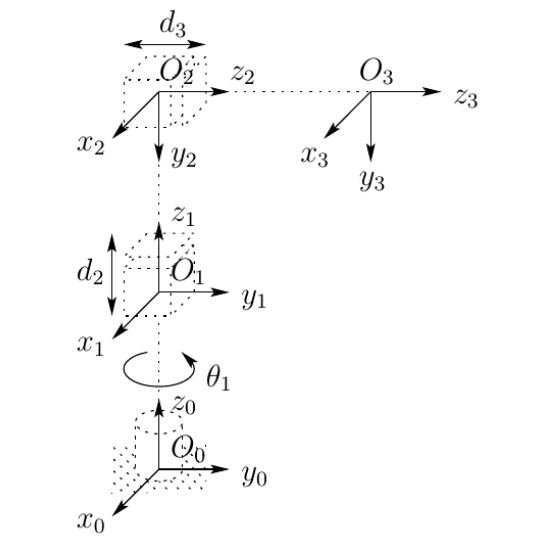
\includegraphics[width=0.47\textwidth]{q4.png}
  \caption{Three link three joint robot}
  \label{fig:q4.1}
\end{figure}
It's frame assignment is shown in Figure \ref{fig:q4.2}. Let the length of link 1 be $l_1$ and the joint variables be $q_1, q_2, q_3$ respectively.
\begin{figure}[h]
  \centering
  \begin{tikzpicture}[x=1cm, y=1cm, z=-0.6cm]
    \draw [dashed, red]       (-3, 0) -- (-3, 3) node [right] {$l_1$};
    \draw [dashed, red]       (-2, 3) -- (-2, 6) node [right] {$q_2$};
    \draw [dashed, red]       (0, 5) -- (3, 5) node [right] {$q_3$};
    % F0
    \draw [->]       (0, 0) -- (0, 1) node [right] {$z_0$};
    \draw            (0, 0) circle (0.15cm);
    \draw [fill]     (0, 0) circle (0.07cm) node [left] {$x_0$};
    % F1
    \draw [->]       (0, 3) -- (0, 4) node [right] {$z_1$};
    \draw            (0, 3) circle (0.15cm);
    \draw [fill]     (0, 3) circle (0.07cm) node [left] {$x_1$};
    % F2
    \draw [->]       (0, 6) -- (1, 6) node [right] {$z_2$};
    \draw            (0, 6) circle (0.15cm);
    \draw [fill]     (0, 6) circle (0.07cm) node [left] {$x_2$};
    % F3
    \draw [->]       (3, 6) -- (4, 6) node [right] {$z_3$};
    \draw            (3, 6) circle (0.15cm);
    \draw [fill]     (3, 6) circle (0.07cm) node [left] {$x_3$};
  \end{tikzpicture}
  \caption{DH frame assignment}
  \label{fig:q4.2}
\end{figure}

\subsubsection*{DH parameters}
The DH parameters for the frames shown in Figure \ref{fig:q4.2} are as follows
\begin{center}
\begin{tabular}{ c | c c c c }
 \hline
 $F_i \to F_j$ & $\theta$ & d & r & $\alpha$ \\
 \hline
 $0 \to 1$ & $q_1$ & $l_1$ & $0$ & $0^{\circ}$ \\
 $1 \to 2$ & $0$   & $q_2$ & $0$ & $-90^{\circ}$ \\
 $2 \to 3$ & $0$   & $q_3$ & $0$ & $0^{\circ}$ \\
 \hline
\end{tabular}
\end{center}

\subsubsection*{Finding transformation $T_{01}, T_{02}, T_{03}$}
Given frame i and frame j with DH parameters [ $\theta$, d, r, $\alpha$ ] the transformation matrix is
\[
  T_{i,j} \equiv Rot_{z,\theta} * Trans_{z, d} * Trans_{x, r} * Rot_{x, \alpha}
\]
\fromlectures
Consider $T_{01}$
\[
  T_{01} \equiv Rot_{z,q_1} * Trans_{z, l_1} * Trans_{x, 0} * Rot_{x, 0^{\circ}}
\]
\[
  T_{01} \equiv \rz{q_1} * \trans{0}{0}{l_1} * \trans{0}{0}{0} * \rx{0^{\circ}}
\]
\[
  T_{01} \equiv \rz{q_1} * \trans{0}{0}{l_1} * \iden * \iden
\]
\[
  T_{01} \equiv \rz{q_1} * \trans{0}{0}{l_1}
\]
\[
  T_{01} \equiv
  \begin{bmatrix}
    cq_1 & -sq_1 & 0 & 0 \\
    sq_1 & cq_1 & 0 & 0 \\
    0 & 0 & 1 & l_1 \\
    0 & 0 & 0 & 1
  \end{bmatrix}
\]
Where $cq_1 \equiv cos(q_1), sq_1 \equiv sin(q_1)$.
Consider $T_{12}$
\[
  T_{12} \equiv Rot_{z, 0} * Trans_{z, q_2} * Trans_{x, 0} * Rot_{x, -90^{\circ}}
\]
\[
  T_{12} \equiv \rz{0} * \trans{0}{0}{q_2} * \trans{0}{0}{0} * \rx{-90^{\circ}}
\]
\[
  T_{12} \equiv \iden * \trans{0}{0}{q_2} * \trans{0}{0}{0} * \rx{-90^{\circ}}
\]
\[
  T_{12} \equiv \trans{0}{0}{q_2} * \rx{-90^{\circ}}
\]
\[
  T_{12} \equiv \trans{0}{0}{q_2}
  *
  \begin{bmatrix}
    1 & 0 & 0 & 0 \\
    0 & 0 & 1 & 0 \\
    0 & -1 & 0 & 0 \\
    0 & 0 & 0 & 1
  \end{bmatrix}
\]
\[
  T_{12} \equiv
  \begin{bmatrix}
    1 & 0 & 0 & 0 \\
    0 & 0 & 1 & 0 \\
    0 & -1 & 0 & q_2 \\
    0 & 0 & 0 & 1
  \end{bmatrix}
\]
Consider $T_{23}$
\[
  T_{23} \equiv Rot_{z, 0} * Trans_{z, q_3} * Trans_{x, 0} * Rot_{x, 0^{\circ}}
\]
\[
  T_{23} \equiv \rz{0} * \trans{0}{0}{q_3} * \trans{0}{0}{0} * \rx{0^{\circ}}
\]
\[
  T_{23} \equiv \iden * \trans{0}{0}{q_3} * \trans{0}{0}{0} * \iden
\]
\[
  T_{23} \equiv \trans{0}{0}{q_3}
\]
But
\[
  T_{ij} \equiv T_{ik} * T_{kj}
\]
\fromlectures
Therefore,
\[
  T_{02} \equiv T_{01} * T_{12}
\]
\[
  T_{02} \equiv
  \begin{bmatrix}
    cq_1 & -sq_1 & 0 & 0 \\
    sq_1 & cq_1 & 0 & 0 \\
    0 & 0 & 1 & l_1 \\
    0 & 0 & 0 & 1
  \end{bmatrix}
  *
  \begin{bmatrix}
    1 & 0 & 0 & 0 \\
    0 & 0 & 1 & 0 \\
    0 & -1 & 0 & q_2 \\
    0 & 0 & 0 & 1
  \end{bmatrix}
\]
\[
  T_{02} \equiv
  \begin{bmatrix}
    cq_1 & 0 & -sq_1 & 0 \\
    sq_1 & 0 & cq_1 & 0 \\
    0 & -1 & 0 & l_1 + q_2 \\
    0 & 0 & 0 & 1
  \end{bmatrix}
\]
\[
  T_{03} \equiv T_{02} * T_{23}
\]
\[
  T_{03} \equiv
  \begin{bmatrix}
    cq_1 & 0 & -sq_1 & 0 \\
    sq_1 & 0 & cq_1 & 0 \\
    0 & -1 & 0 & l_1 + q_2 \\
    0 & 0 & 0 & 1
  \end{bmatrix}
  *
  \trans{0}{0}{q_3}
\]
\[
  T_{03} \equiv
  \begin{bmatrix}
    cq_1 & 0 & -sq_1 & -q_3sq_1 \\
    sq_1 & 0 &  cq_1 &  q_3cq_1 \\
    0 & -1 & 0 & l_1 + q_2 \\
    0 & 0 & 0 & 1
  \end{bmatrix}
\]

\subsubsection*{Finding Jacobian}
For an RPP robot, the Jacobian of pose of end effector w.r.t frame 0 as a function of joint variables
\[
  J \equiv
  \begin{bmatrix}
    z_0^0 \times a_{03}^0 & z_1^0 & z_2^0 \\
    z_0^0 & 0 & 0
  \end{bmatrix}
\]
where
\[
  a_{i3}^{0} \equiv a_{3}^{0} - a_{i}^{0}
\]
where $a_3^0$ is the origin of frame 3 in frame 0 and $a_i^0$ is origin of frame i in frame 0.
$z_i^0$ can be obtained by the first three number of third column of $T_{0i}$.
\fromlectures
\[
  z_0^0 \equiv z_1^0 \equiv \begin{bmatrix}
    0 \\
    0 \\
    1
  \end{bmatrix}
\]
\[
  z_2^0 \equiv
  \begin{bmatrix}
    -sq_1 \\
     cq_1 \\
     0
  \end{bmatrix}
\]
Consider $a_3^0$,
\[
  a_3^0 \equiv T_{03} * O_3
\]
\[
  a_3^0 \equiv
  \begin{bmatrix}
    cq_1 & 0 & -sq_1 & -q_3sq_1 \\
    sq_1 & 0 &  cq_1 &  q_3cq_1 \\
    0 & -1 & 0 & l_1 + q_2 \\
    0 & 0 & 0 & 1
  \end{bmatrix}
  *
  \begin{bmatrix}
    0 \\
    0 \\
    0 \\
    1
  \end{bmatrix}
\]
\[
  a_3^0 \equiv
  \begin{bmatrix}
    -q_3sq_1 \\
    q_3cq_1 \\
    l_1 + q_2 \\
    1
  \end{bmatrix}
\]
Removing the homogeneous coordinate,
\[
  a_3^0 \equiv
  \begin{bmatrix}
    -q_3sq_1 \\
    q_3cq_1 \\
    l_1 + q_2
  \end{bmatrix}
\]
Consider $a_0^0$,
\[
  a_0^0 \equiv \begin{bmatrix}
    0 \\
    0 \\
    0
  \end{bmatrix}
\]
Therefore,
\[
  a_{03}^0 \equiv
  \begin{bmatrix}
    -q_3sq_1 \\
    q_3cq_1 \\
    l_1 + q_2
  \end{bmatrix}
\]
Consider
\[
  z_0^0 \times a_{03}^0 \equiv
  \begin{bmatrix}
    0 \\
    0 \\
    1
  \end{bmatrix}
  \times
  \begin{bmatrix}
    -q_3sq_1 \\
    q_3cq_1 \\
    l_1 + q_2
  \end{bmatrix}
  \equiv
  \begin{bmatrix}
    -q_3cq_1 \\
    -q_3sq_1 \\
    0
  \end{bmatrix}
\]
Using these quantities to build the Jacobian,
\[
  J \equiv
  \begin{bmatrix}
    z_0^0 \times a_{03}^0 & z_1^0 & z_2^0 \\
    z_0^0 & 0 & 0
  \end{bmatrix}
\]
\[
  J \equiv
  \begin{bmatrix}
    -q_3cq_1 & 0 & -sq_1 \\
    -q_3sq_1 & 0 &  cq_1 \\
    0        & 1 &  0 \\
    0 & 0 & 0 \\
    0 & 0 & 0 \\
    1 & 0 & 0
  \end{bmatrix}
\]

\end{document}
